% ECE 285 HW2 -- two-page NeurIPS-format report.
\documentclass{article}
\usepackage[preprint,nonatbib]{neurips_2024}
\usepackage[T1]{fontenc}
\usepackage[utf8]{inputenc}
\usepackage{amsmath,amssymb,graphicx,booktabs}
\usepackage[hidelinks]{hyperref}
\setlength{\textfloatsep}{7pt plus 2pt minus 2pt}
\setlength{\floatsep}{5pt plus 2pt minus 2pt}
\setlength{\intextsep}{5pt plus 2pt minus 2pt}
\setlength{\abovecaptionskip}{3pt}
\setlength{\belowcaptionskip}{-2pt}
\setlength{\abovedisplayskip}{3pt plus 1pt minus 1pt}
\setlength{\belowdisplayskip}{3pt plus 1pt minus 1pt}

\begin{document}

\begin{center}
\rule{\linewidth}{1.2pt}\\[7pt]
{\LARGE\bfseries Unconditional GANs for WikiArt Paintings}\\[6pt]
{\large Xiyin Xu}\\[3pt]
{\small Code and results: \href{https://github.com/CiciAa777/285hw2-gan}{\texttt{github.com/CiciAa777/285hw2-gan}}}\\[3pt]
\rule{\linewidth}{0.6pt}
\end{center}
\vspace{-5pt}

\section{Model and Hyperparameter Settings}
We train an unconditional DCGAN~\cite{dcgan} on the WikiArt dataset~\cite{wikiart}. The processed set contains 81,444 valid $64\times64$ RGB paintings in 27 style folders. We pool all folders without using style labels and make a deterministic 95/5 split (77,371 train; 4,073 held-out) with seed 42. Images are fit to a square, converted to RGB, and scaled to $[-1,1]$; augmentation is disabled.

The generator maps $z\sim\mathcal N(0,I)$, $z\in\mathbb R^{100}$, through a learned projection and four transposed-convolution upsampling stages (512, 256, 128, 64 channels) to an RGB image with a $\tanh$ output. The discriminator mirrors this with four stride-2 convolution stages (64, 128, 256, 512 channels) and one real/fake logit. Generator hidden layers use batch normalization and ReLU; discriminator layers use LeakyReLU, with batch normalization after the first block. We use DCGAN normal initialization and binary cross-entropy with logits.

\begin{table}[!ht]
\centering
\caption{Shared setup and the main training hyperparameters. Trial-specific changes are listed in Table~\ref{tab:results}.}
\label{tab:setup}
\small
\setlength{\tabcolsep}{4pt}
\begin{tabular}{@{}ll@{}}
\toprule
Data / split & 81,444 images; 77,371 train / 4,073 held-out; seed 42 \\
Preprocessing & RGB, square fit, $64^2$, values in $[-1,1]$, no augmentation \\
Architecture & DCGAN; $z=100$; base channels 64; G: BN/ReLU; D: LeakyReLU \\
Optimization & BCE-with-logits; Adam, $\beta=(0.5,0.999)$; 50 epochs \\
Learning rates & $\mathrm{lr}_G=2\times10^{-4}$; $\mathrm{lr}_D\in\{2,1,0.5\}\times10^{-4}$ \\
Update ratio & 1 G step per D step, except Trial 4 (2 G steps) \\
Compute & DSMLP medium-class CUDA GPUs; batch 64 unless noted \\
\bottomrule
\end{tabular}
\end{table}

\section{Training Loss Curves}
Figure~\ref{fig:loss} plots per-epoch means from all minibatches for Trial 2, which attained the highest IS. The discriminator loss falls quickly while generator loss rises, indicating an increasingly strong discriminator under this BCE objective. These adversarial losses are not direct measures of perceptual image quality.
\begin{figure}[!ht]
\centering
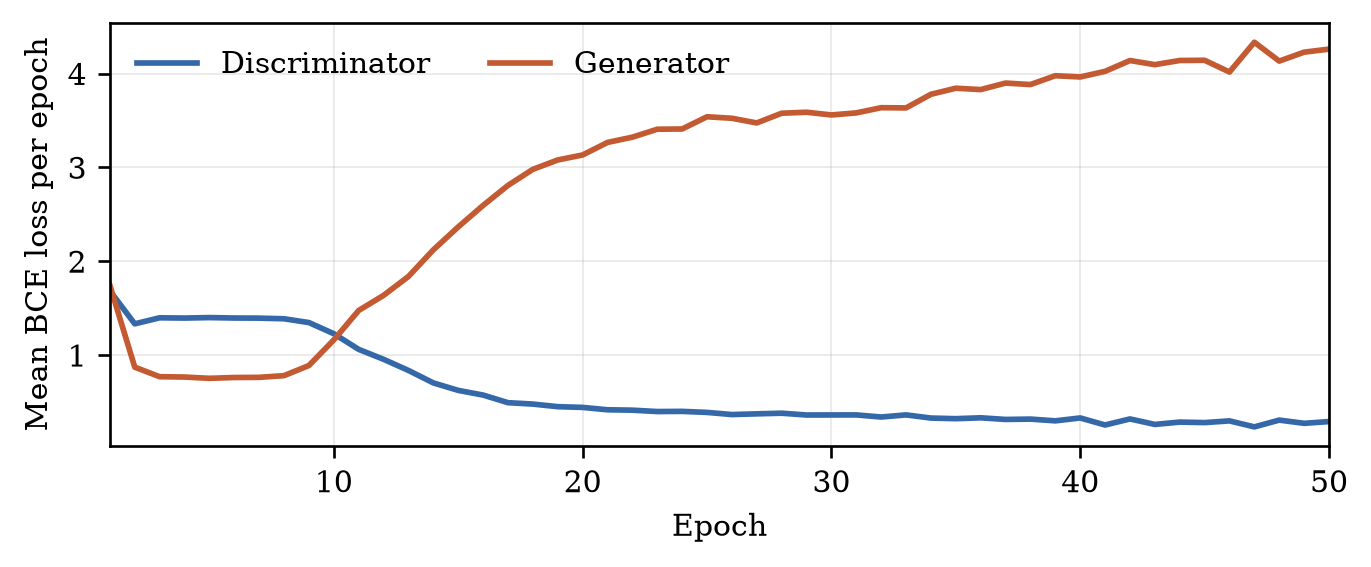
\includegraphics[width=.78\linewidth]{figures/trial2_losses.png}
\caption{Trial 2 (batch 64, $\mathrm{lr}_D=5\times10^{-5}$), averaged by epoch.}
\label{fig:loss}
\end{figure}

\section{FID/IS Scores and Hyperparameter Results}
We follow the PyTorch-Ignite evaluation workflow~\cite{ignite}, comparing 4,073 generated images with the 4,073 held-out paintings. Both sets are resized to $299\times299$ for Inception metrics. IS uses generated images only~\cite{is}, whereas FID compares generated and real feature distributions~\cite{fid}; both depend on an ImageNet-trained classifier and are imperfect measures of artwork quality. Values below are single-run estimates without uncertainty intervals.

\begin{table}[!ht]
\centering
\caption{Completed experiments, all trained for 50 epochs. Higher IS and lower FID are preferred; best observed values are bold.}
\label{tab:results}
\footnotesize
\setlength{\tabcolsep}{3pt}
\begin{tabular}{@{}l p{2.55in} c r r@{}}
\toprule
Run & Change & Batch & IS $\uparrow$ & FID $\downarrow$ \\
\midrule
Baseline & DCGAN; $\mathrm{lr}_D=2\times10^{-4}$ & 64 & 2.525 & .0792 \\
Trial 1 & $\mathrm{lr}_D=10^{-4}$ & 64 & 2.684 & \textbf{.0372} \\
Trial 2 & $\mathrm{lr}_D=5\times10^{-5}$ & 64 & \textbf{2.951} & .0424 \\
Trial 3 & Batch-size change from Trial 2 & 32 & 2.118 & .1165 \\
Trial 4 & Two G updates per D update (Trial 3 base) & 32 & 2.807 & .1631 \\
Trial 5 & Spectral normalization on D (Trial 2 base) & 64 & 2.295 & .0987 \\
\bottomrule
\end{tabular}
\end{table}

Reducing the discriminator learning rate improved the baseline: Trial 1 had the lowest FID, while Trial 2 had the highest IS. Trial 3's smaller batch and Trial 5's spectral normalization both lowered scores relative to Trial 2. Trial 4 raised IS over Trial 3 but had the largest FID, so its 2:1 G:D update ratio gave no consistent gain. Trial 2 is the balanced example checkpoint (highest IS, near-best FID); Trial 1 remains the FID leader. Overall, balancing discriminator strength mattered more than the tested update-ratio and regularization changes.

\section{Generated Painting Examples}
Figure~\ref{fig:samples} shows fixed-noise grids from the two strongest runs by complementary metrics. The outputs capture painterly color fields and textured brush-like patterns, but often blur forms together and repeat motifs. The $64\times64$ resolution limits detail, and the unconditional model does not control style.
\begin{figure}[!ht]
\centering
\begin{minipage}{.485\linewidth}\centering
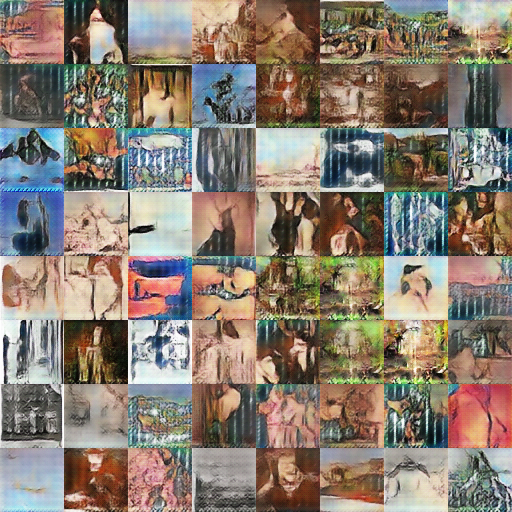
\includegraphics[width=.86\linewidth]{figures/trial1_grid.png}\\[-1pt]
{\small (a) Trial 1: best FID}
\end{minipage}\hfill
\begin{minipage}{.485\linewidth}\centering
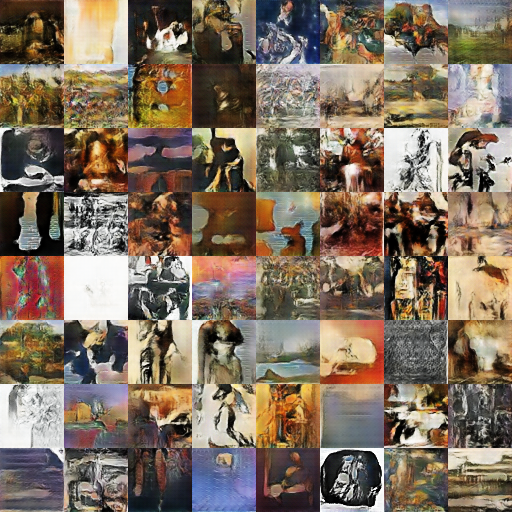
\includegraphics[width=.86\linewidth]{figures/trial2_grid.png}\\[-1pt]
{\small (b) Trial 2: best IS}
\end{minipage}
\caption{64 generated samples per checkpoint, arranged as fixed-noise grids.}
\label{fig:samples}
\end{figure}

\paragraph{Limitations.} These metrics are computed once and inherit ImageNet-domain bias; results are not averaged across training seeds. Larger images, repeated seeds, and capacity or activation ablations would clarify whether the observed ranking is robust.

\begin{thebibliography}{5}
\footnotesize
\bibitem{dcgan} A. Radford, L. Metz, and S. Chintala. Unsupervised Representation Learning with Deep Convolutional Generative Adversarial Networks. ICLR, 2016.
\bibitem{wikiart} Steubk. \href{https://www.kaggle.com/datasets/steubk/wikiart}{WikiArt dataset}. Kaggle.
\bibitem{ignite} PyTorch-Ignite. \href{https://pytorch-ignite.ai/blog/gan-evaluation-with-fid-and-is/}{GAN evaluation using FID and IS}.
\bibitem{is} T. Salimans et al. Improved Techniques for Training GANs. NeurIPS, 2016.
\bibitem{fid} M. Heusel et al. GANs trained by a two time-scale update rule. NeurIPS, 2017.
\end{thebibliography}
\end{document}
